\documentclass[
a5paper,
10pt, 
onecolumn,
openany,
]{memoir}

\usepackage{fontspec}
\usepackage[raggedright,bf,sf]{titlesec}
\usepackage{titletoc}
\usepackage{titling}
\usepackage{nameref}
\usepackage[german]{babel} % English please
\usepackage[final]{microtype} % Less badboxes
\usepackage{graphicx} % Include figures
\usepackage{lipsum} % Just to put in some text
\usepackage{xcolor}
\usepackage{caption}

\usepackage{merriweather}
\usepackage{librecaslon} % Caslon font

\setmainfont{Libre Caslon Text}
%\setsansfont{Merriweather Sans}
\setsansfont{Myriad Pro}

\renewcommand{\printtoctitle}[1]{\LARGE\sffamily #1}
\renewcommand{\printloftitle}[1]{\LARGE\sffamily #1}
\renewcommand{\printlottitle}[1]{\LARGE\sffamily #1}

\titlecontents{chapter}
  [1.5em] % ie, 1.5em (chapter) + 2.3em
  {\sffamily}
  {\contentslabel{2.3em}}
  {\hspace*{-2.3em}}
  {\titlerule*[1pc]{.}\contentspage}

\titlecontents{subsection}
  [6.1em] % ie, 1.5em (chapter) + 2.3em
  {\sffamily}
  {\contentslabel{2.3em}}
  {\hspace*{-2.3em}}
  {\titlerule*[1pc]{.}\contentspage}

\titlecontents{section}
  [3.8em] % ie, 1.5em (chapter) + 2.3em
  {\sffamily}
  {\contentslabel{2.3em}}
  {\hspace*{-2.3em}}
  {\titlerule*[1pc]{.}\contentspage}

\newcommand{\tabref}[1]{Tabelle \ref{#1}: \nameref{#1}}

\captionsetup{%
  font={normalsize}, % small font size
  labelfont={sf},      % label in bold, sans-serif
  textfont={sf},
  singlelinecheck=true, % centered single-lined captions
  format=plain,             % indention=1cm,
  labelsep={colon},         % default separator: none, colon, period, space, quad, newline, endash
}

%\titleformat{\chapter}[display]{\sffamily\Huge}{}{1em}{\thechapter}
\titleformat{\chapter}[display]{\sffamily\LARGE}{\raggedleft\HUGE\textcolor{gray}{\normalfont\thechapter}}{0.5em}{}[\titlerule]
\titleformat*{\section}{\sffamily\LARGE}
\titleformat*{\subsection}{\sffamily\Large}
\titleformat*{\subsubsection}{\sffamily\large}
\titleformat*{\paragraph}{\sffamily\large}
\titleformat*{\subparagraph}{\sffamily\large}

\setlrmarginsandblock{0.15\paperwidth}{*}{1} % Left and right margin
\setulmarginsandblock{0.2\paperwidth}{*}{1}  % Upper and lower margin
\checkandfixthelayout

\maxsecnumdepth{subsection} % Subsections (and higher) are numbered
\setsecnumdepth{subsection}

\chapterstyle{standard}

\makeatletter                  % You do not need to write [htpb] all the time
\renewcommand\fps@figure{htbp} %
\renewcommand\fps@table{htbp}  %
\makeatother                   %

%%% HEADER AND FOOTER 
%%%------------------------------------------------------------------------------

\makepagestyle{standard} % Make standard pagestyle

\makeatletter                 % Define standard pagestyle
\makeevenfoot{standard}{\small\sffamily\thepage}{}{} %
\makeoddfoot{standard}{}{}{\small\sffamily\thepage}  %
\makeevenhead{standard}{\textcolor{gray}{\sffamily\small\leftmark}}{}{}
\makeoddhead{standard}{}{}{\textcolor{gray}{\sffamily\small\rightmark}}
\makeheadrule{standard}{\textwidth}{\normalrulethickness}
\makeatother                  %

\makeatletter
\makepsmarks{standard}{
\createmark{chapter}{both}{shownumber}{\@chapapp\ }{ \quad }
\createmark{section}{right}{shownumber}{}{ \quad }
\createplainmark{toc}{both}{\contentsname}
\createplainmark{lof}{both}{\listfigurename}
\createplainmark{lot}{both}{\listtablename}
\createplainmark{bib}{both}{\bibname}
\createplainmark{index}{both}{\indexname}
\createplainmark{glossary}{both}{\glossaryname}
}
\makeatother                               %

\makepagestyle{chap} % Make new chapter pagestyle

\makeatletter
\makeevenfoot{chap}{\small\sffamily\thepage}{}{} % Define new chapter pagestyle
\makeoddfoot{chap}{}{}{\small\sffamily\thepage}  %
\makeevenhead{chap}{}{}{}   %
\makeoddhead{chap}{}{}{}    %
%\makeheadrule{chap}{\textwidth}{\normalrulethickness}
\makeatother

\nouppercaseheads
\pagestyle{standard}               % Choosing pagestyle and chapter pagestyle
\aliaspagestyle{chapter}{chap} %

\maxtocdepth{subsection} % Only parts, chapters and sections in the table of contents
\settocdepth{subsection}

\author{\sffamily\huge A. Author}
\title{\sffamily\Huge The amazing Book about Timemachines}
\date{}

\begin{document}

\frontmatter

\maketitle

\clearpage

\tableofcontents*

\clearpage

\chapter{Vorwort}

\lipsum[1-2]

\begin{figure}
  \centering
  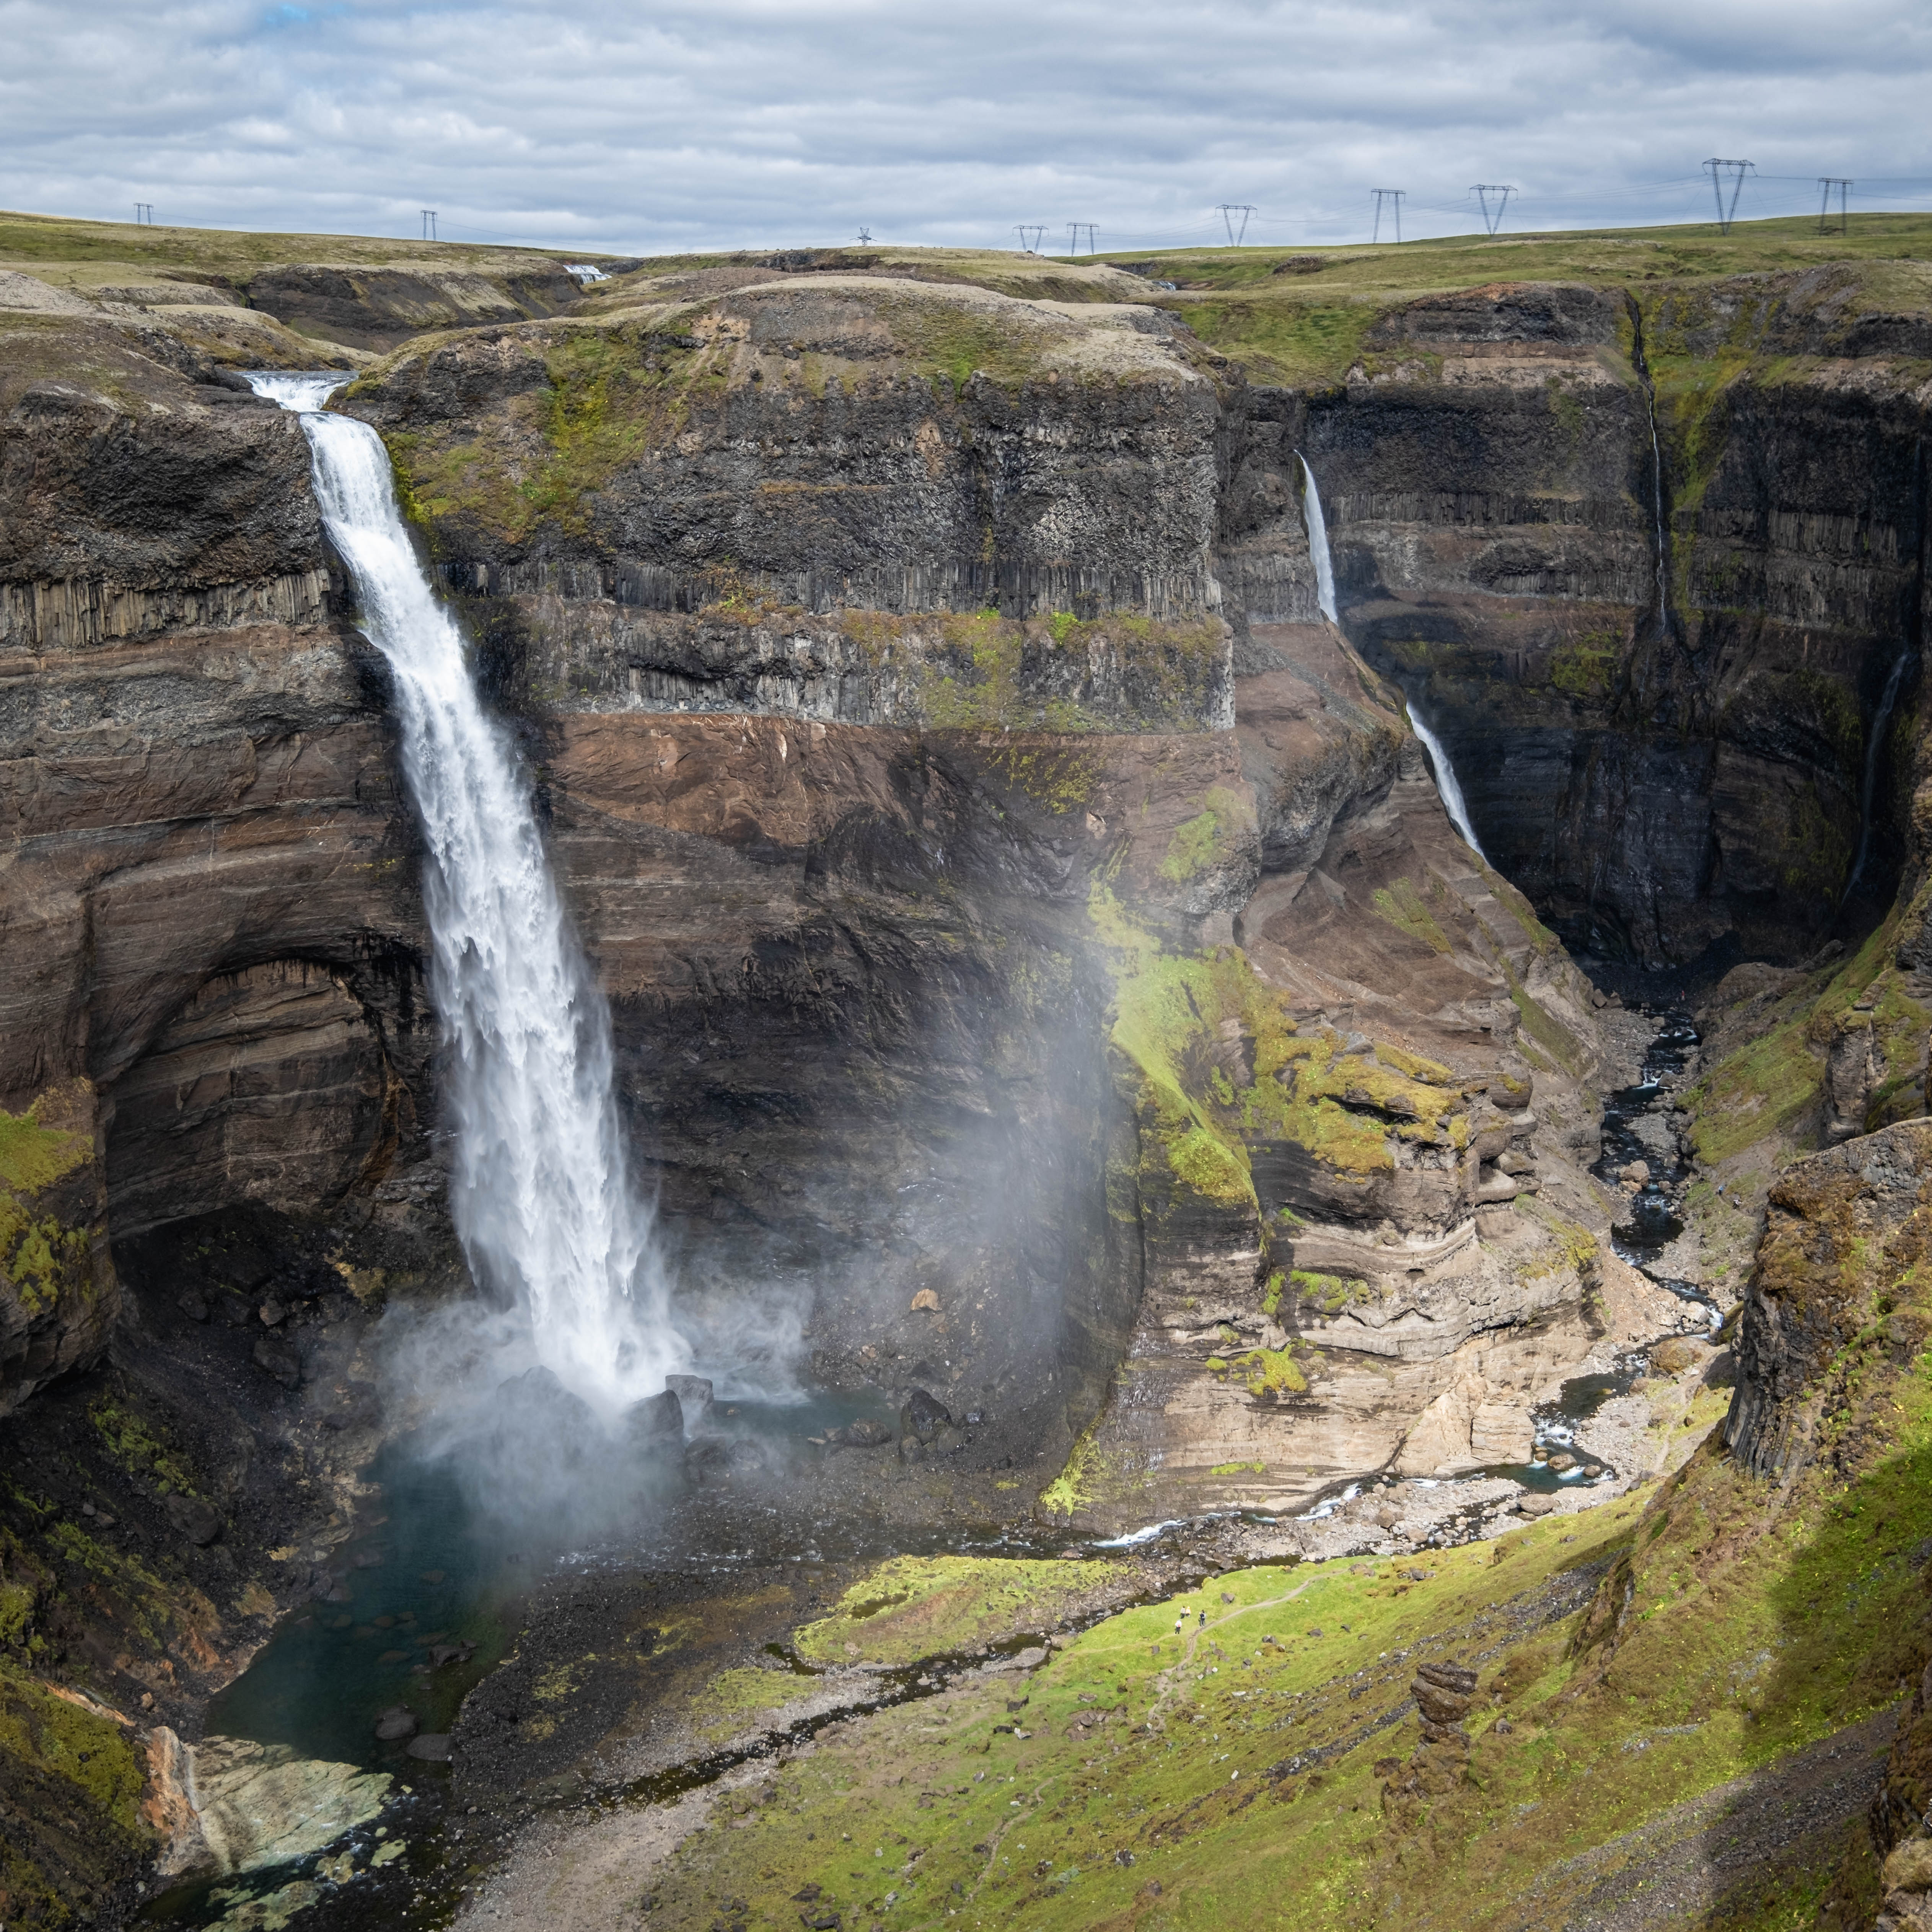
\includegraphics[width=0.9\textwidth]{fotos/a}
  \caption{Ein Bär}
\end{figure}

\lipsum[1-2]

\mainmatter

\chapter{Wie man eine Zeitmaschine baut}

\lipsum[1-1] 

\section{Anforderungen}

\lipsum[1-1]

\begin{table}
  \centering
  \begin{tabularx}{0.9\textwidth}{ c l l X }
    Jahr & Name & Partner & \\
    \hline\noalign{\smallskip}
    1906 & Peter Pan & Petra & toller König \\ 
    1907 & Max Müller & Mimi &  \\  
    1908 & Susi Sommer & Simon & erste Frau \\
    1906 & Peter Pan & Petra & toller König \\ 
    1907 & Max Müller & Mimi &  \\  
    1907 & Max Müller & Mimi &  \\  
    1908 & Susi Sommer & Simon & erste Frau \\
    1906 & Peter Pan & Petra & toller König \\ 
    1907 & Max Müller & Mimi &  \\  
    1908 & Susi Sommer & Simon & erste Frau \\
  \end{tabularx}
  \caption{Könige historisch}
  \label{fig:tab_koenige_historisch}
\end{table}

\section{Ausführung}

\lipsum[1-1]

\begin{figure}
  \centering
  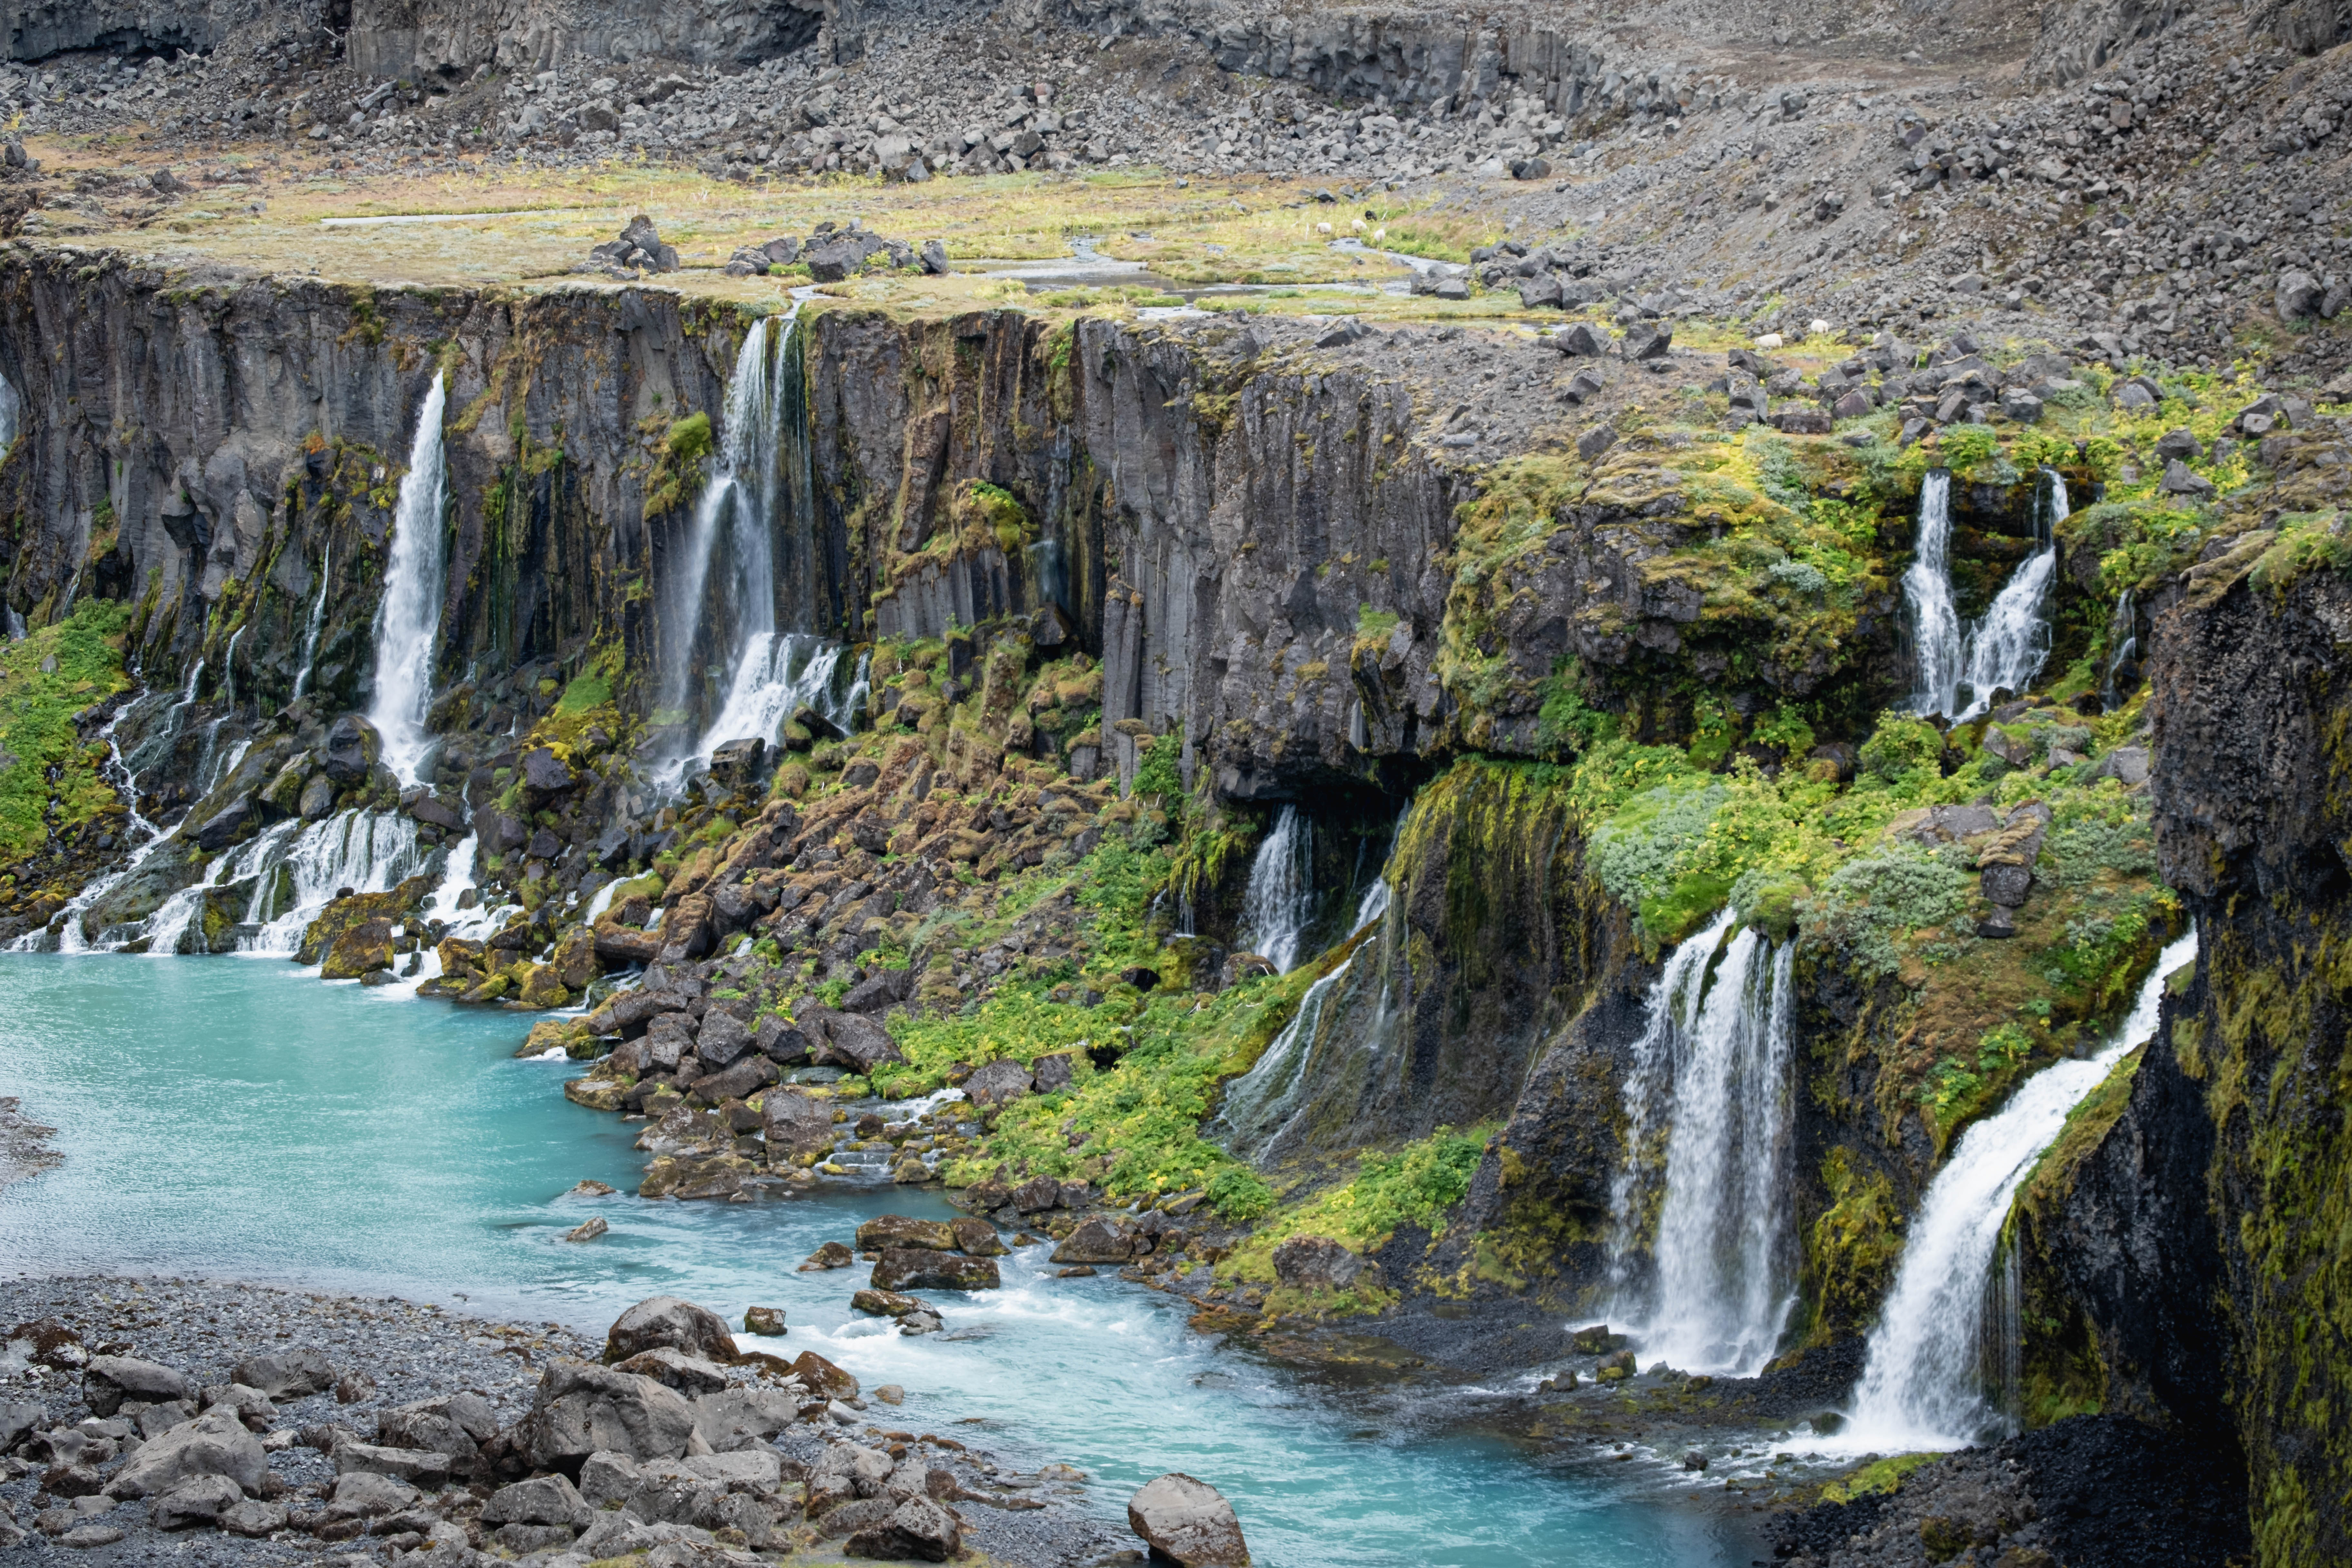
\includegraphics[width=0.3\textwidth]{fotos/b}
  \caption{Noch ein Bär}
\end{figure}

\lipsum[1-4]

\chapter{Wie man eine Zeitmaschine zerstört}

\lipsum[1-3]

\section{Ausrüstung}

Jemand musste Josef K. verleumdet haben, denn ohne dass er etwas Böses getan hätte, wurde er eines Morgens verhaftet. »Wie ein Hund! « sagte er, es war, als sollte die Scham ihn überleben. Als Gregor Samsa eines Morgens aus unruhigen Träumen erwachte, fand er sich in seinem Bett zu einem ungeheueren Ungeziefer verwandelt.

Und es war ihnen wie eine Bestätigung ihrer neuen Träume und guten Absichten, als am Ziele ihrer Fahrt die Tochter als erste sich erhob und ihren jungen Körper dehnte. »Es ist ein eigentümlicher Apparat«, sagte der Offizier zu dem Forschungsreisenden und überblickte mit einem gewissermaßen bewundernden Blick den ihm doch wohlbekannten Apparat.
%TODO mehr platz?

Sie hätten noch ins Boot springen können, aber der Reisende hob ein schweres, geknotetes Tau vom Boden, drohte ihnen damit und hielt sie dadurch von dem Sprunge ab. In den letzten Jahrzehnten ist das Interesse (siehe \tabref{fig:tolle_tabelle}) an Hungerkünstlern sehr zurückgegangen. Aber sie überwanden sich, umdrängten den Käfig und wollten sich gar nicht fortrühren. Jemand musste Josef K. verleumdet haben, denn ohne dass er etwas Böses getan hätte, wurde er eines Morgens verhaftet. »Wie ein Hund! « sagte er, es war, als sollte die Scham ihn überleben. Als Gregor Samsa eines Morgens aus unruhigen Träumen erwachte, fand er sich

\section{Erfahrung}

\lipsum[1-1]

\section{Testergebnisse}

\lipsum[1-1]

\subsection{Test 1}

Test fehlgeschlagen

\subsection{Test 2}

\begin{table}
\centering
\begin{tabularx}{0.9\textwidth}{l | c X}
abc & asd & gfdf g \\
asjdlasd & as  d & sd546dfg \\
asjda & dfhjsdf & flkhgölf kgh \\
\end{tabularx}
\caption{Testergebnisse}
\label{fig:tolle_tabelle}
\end{table}

\subsection{Schulisch}

\begin{figure}
  \centering
  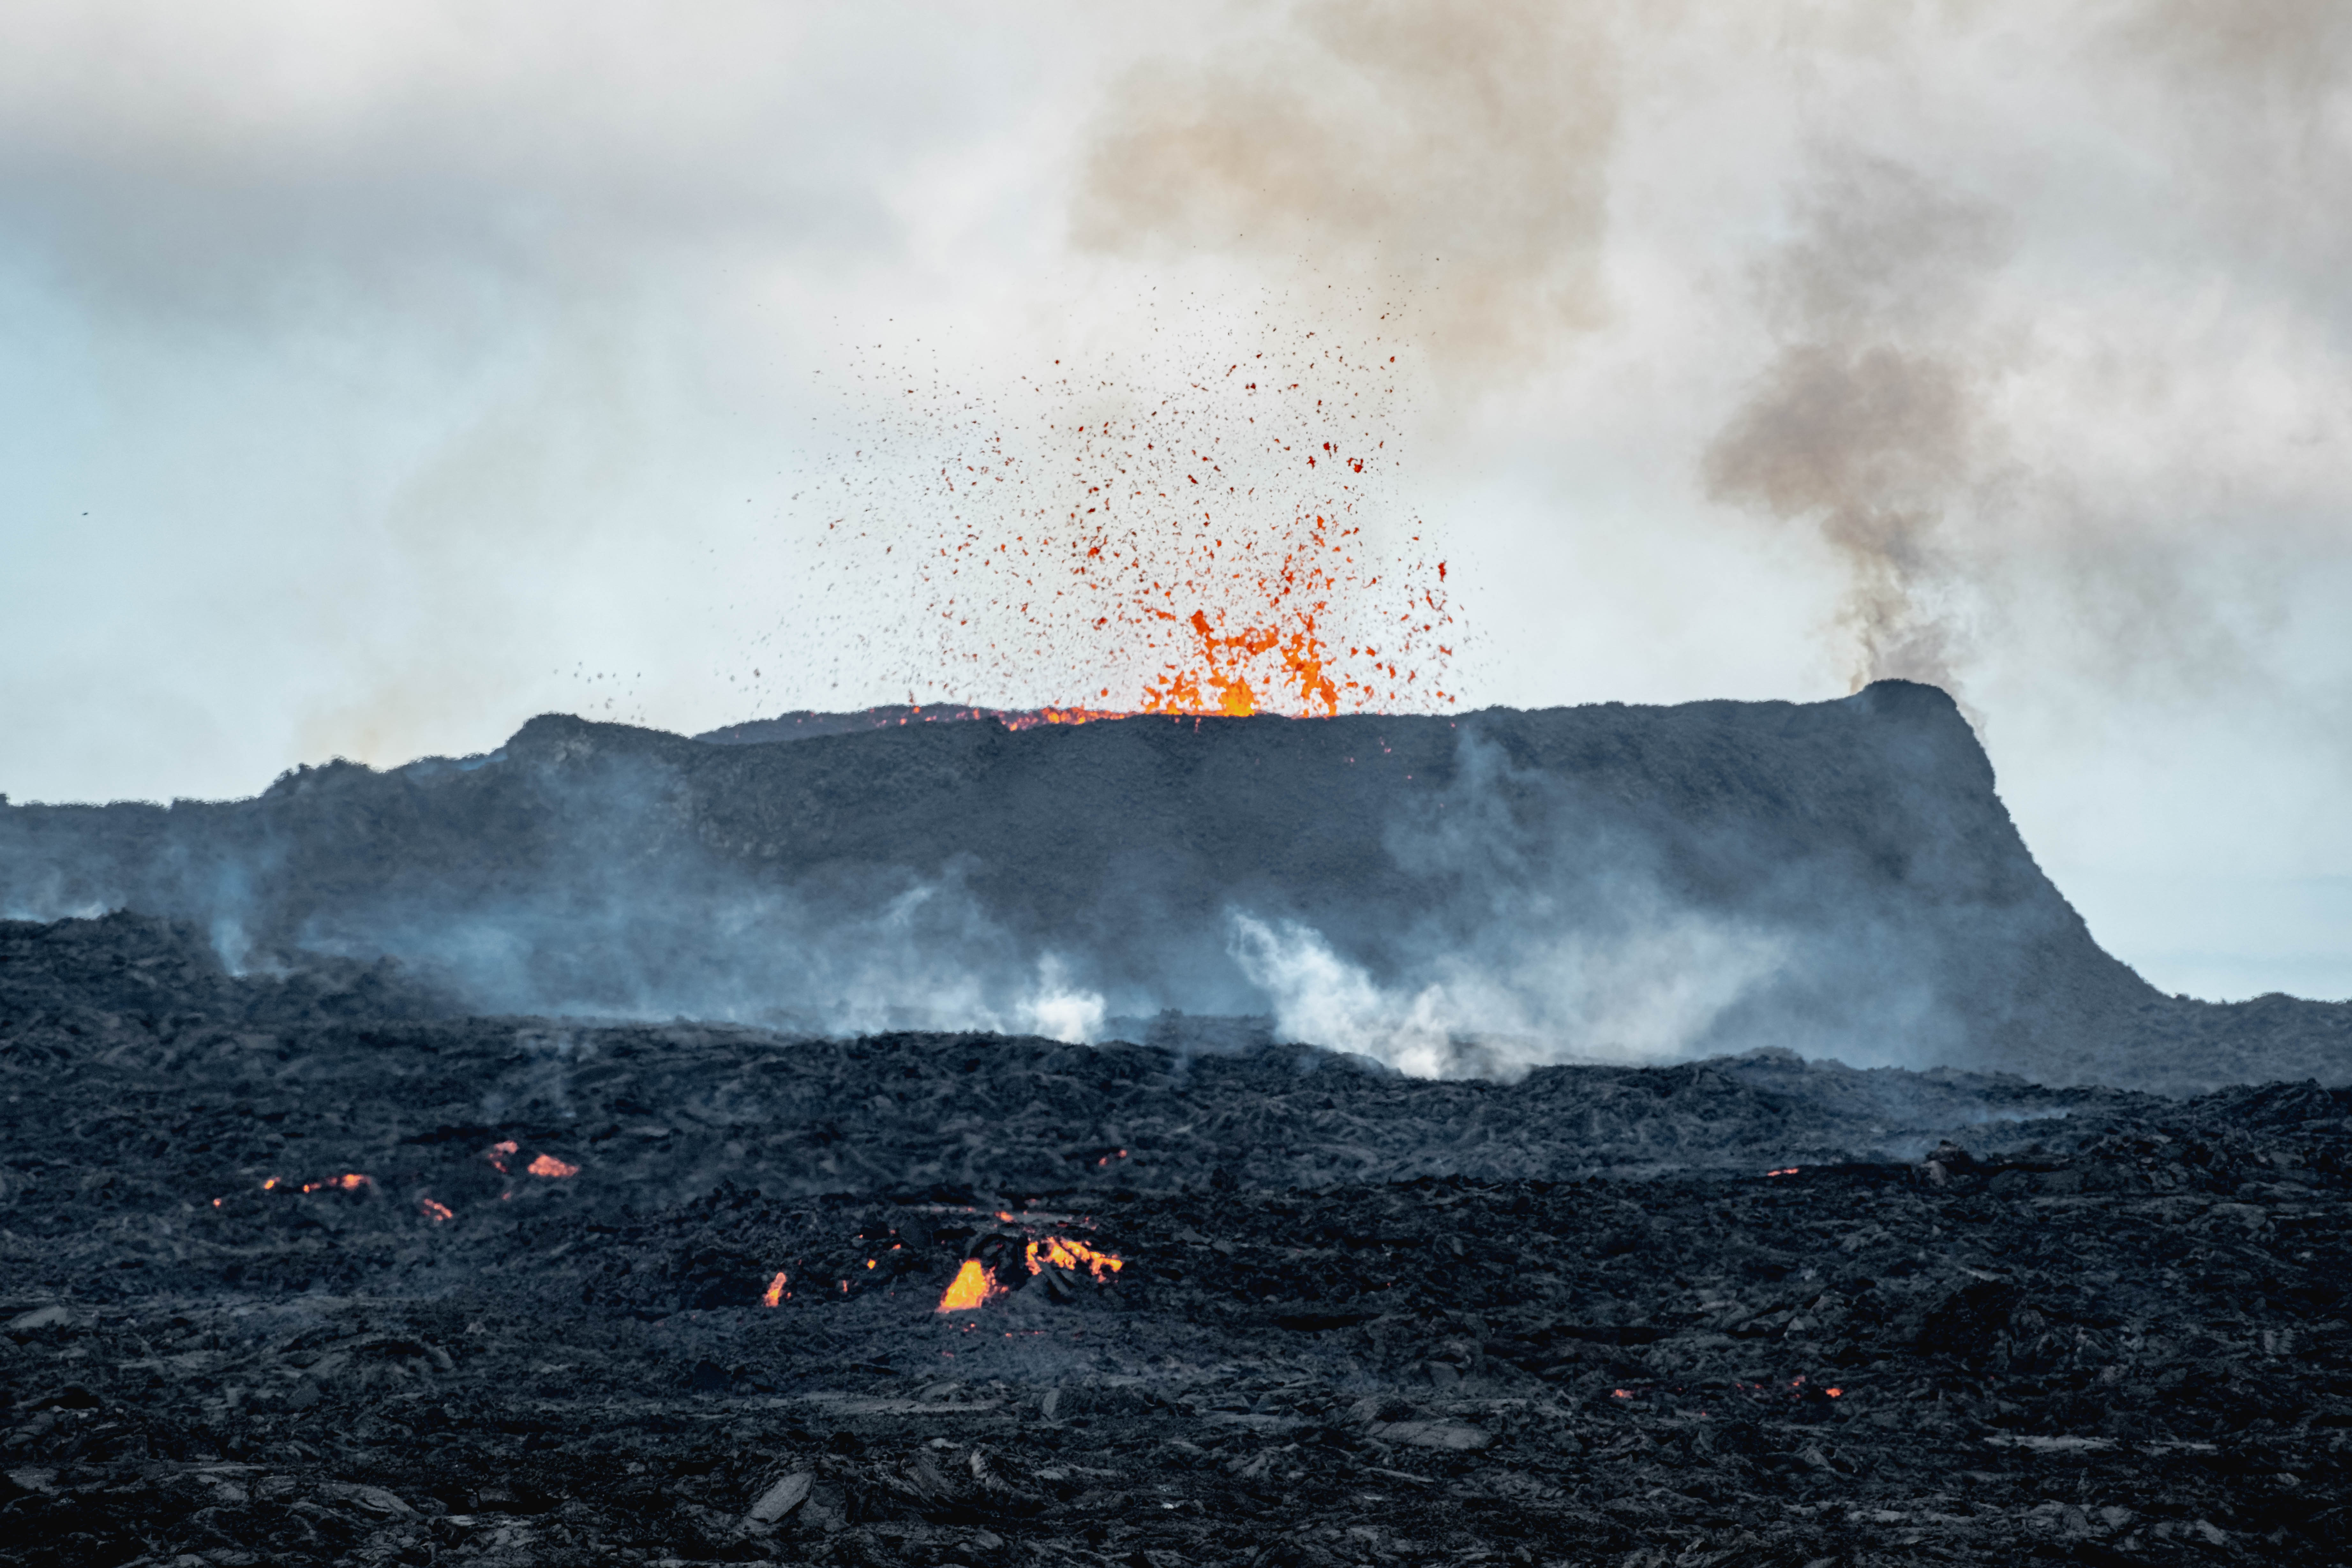
\includegraphics[width=0.8\textwidth]{fotos/d}
  \caption{Mehr Bär}
\end{figure}

\lipsum[1-5]

\subsection{Arbeitsumfeld}

\lipsum[1-2]

\clearpage
 
\thispagestyle{empty}
\listoffigures
\clearpage

\thispagestyle{empty}
\listoftables
\clearpage

\appendix

\chapter{Kausalität}

\lipsum[1-2]

\backmatter

\end{document}